\documentclass[a4paper]{article}
\usepackage{pdp}
\title{Othello -- Python}
\subtitle{Rapport Préliminaire}
\author{
    Grégory Bonzon,
    Rémi Boussion,
    Gabriel Ringuet,
    Matthieu Vigier-Lafosse,
    Arthur Voisin
}

\begin{document}
\maketitle
\thispagestyle{empty}


\section{Explication détaillée du sujet}

\subsection{Historique et Règles}
Le projet consiste à développer le jeu de société Othello, un jeu de stratégie combinatoire abstrait à information parfaite, inventé sous sa forme moderne au XIXe siècle et popularisé dans les années 1970. Le jeu se déroule sur un tablier de 8 × 8 cases avec 64 pions bicolores, où l'objectif est de posséder la majorité des pions à la fin de la partie. Les Noirs ouvrent toujours le jeu, puis les participants posent tour à tour une pièce de leur couleur en respectant une règle de capture stricte : chaque coup doit obligatoirement « prendre en sandwich » un ou plusieurs pions adverses entre le pion posé et un autre déjà présent, ce qui a pour effet de retourner les pions encadrés pour qu'ils prennent la couleur du joueur actif. Si un joueur ne peut effectuer aucune prise, il doit passer son tour jusqu'à ce que le plateau soit plein ou qu'aucun coup ne soit possible. Une stratégie fondamentale consiste à viser prioritairement les quatre coins du plateau, car un pion placé dans un coin est imprenable et permet de stabiliser durablement ses lignes tout en bloquant les opportunités de l'adversaire.

\subsection{Complexité du Jeu}
Othello possède une complexité d'espace d'états estimée à environ $10^{28}$ positions légales, ce qui est inférieur aux échecs ($10^{46}$) mais reste suffisamment vaste pour nécessiter des algorithmes d'intelligence artificielle performants \cite{rosenbloom, lee}. Des travaux plus récents sur l'apprentissage automatique, comme le programme Logistello, ont démontré l'importance des stratégies d'ouverture et de fin de partie \cite{buro}.

\section{Algorithmes et Structures de Données}

Pour garantir la performance exigée par le cahier des charges (notamment pour l'IA et le mode \textit{Contest}), nous avons choisi des structures optimisées.
\subsection{Gestion de l'Historique : Piles}

Pour répondre au besoin d'annulation et de rétablissement des coups (fonctionnalité F12), nous intégrons deux structures de données de type Pile au sein de l'état du jeu.

\begin{itemize}
    \item \textbf{Pile d'Historique (\texttt{undo\_stack}) :} Avant chaque modification de l'état du jeu (jouer un coup), une copie de l'état courant est empilée.
    \item \textbf{Pile de Rétablissement (\texttt{redo\_stack}) :} Lorsqu'un joueur annule un coup, l'état restauré est transféré de la pile d'historique vers cette pile de rétablissement. Cela permet de revenir vers le futur si le joueur change d'avis.
\end{itemize}

\textbf{Cohérence :} Il est important de noter que si un joueur effectue un \textit{nouveau} coup alors que la pile \texttt{redo\_stack} n'est pas vide, cette dernière est vidée. En effet, jouer un nouveau coup crée une nouvelle branche dans l'historique, invalidant les états futurs précédemment stockés.

\subsection{Représentation du Plateau : Bitboards}
Au lieu d'utiliser un tableau à deux dimensions (ex: \texttt{int board[8][8]}), nous utiliserons des Bitboards (entiers de 64 bits).

\begin{itemize}
    \item \textbf{Justification :} Cette structure permet de représenter l'ensemble des pions d'un joueur en un seul entier \cite{Browne2014} (\texttt{uint64}). Les opérations logiques (\texttt{AND}, \texttt{OR}, \texttt{XOR}, \texttt{SHIFT}) permettent de calculer les coups légaux et les retournements en parallèle sur tout le plateau, offrant un gain de temps considérable par rapport à une itération case par case.
    \item \textbf{Implémentation :} Le module \texttt{BitboardOps} (voir architecture) gérera les opérations de bas niveau (\texttt{set\_disk}, \texttt{popcount} pour le score, décalages pour explorer les 8 directions).
\end{itemize}
\begin{multicols}{2}
\begin{lstlisting}[title=Algorithme de retournement,
    numbers=none,
    xleftmargin=0pt,
    breaklines=true
]
FONCTION compute_flips(own_board, enemy_board, x, y)
    // 1. Initialisation
    masque_retournements_total = 0
    // Liste des 8 directions (dx, dy)
    directions = [(-1, -1), (-1, 0), (-1, 1), 
                  (0, -1),           (0, 1), 
                  (1, -1),  (1, 0),  (1, 1)]
    // 2. Vérification préalable
    SI la case (x, y) n'est pas vide OU hors plateau ALORS
        RETOURNER 0
    FIN SI
    // 3. Boucle principale
    POUR CHAQUE (dx, dy) DANS directions FAIRE :
        x_courant = x + dx
        y_courant = y + dy
        masque_direction = 0  
        TANT QUE est_dans_grille(x_courant, y_courant) FAIRE :
            index = (y_courant * 8) + x_courant
            bit_mask = 1 << index // Décalage binaire
            // CAS A : Pion ADVERSE
            SI (enemy_board ET bit_mask) != 0 ALORS
                masque_direction = masque_direction OU bit_mask
                x_courant = x_courant + dx
                y_courant = y_courant + dy
            // CAS B : Pion À NOUS
            SINON SI (own_board ET bit_mask) != 0 ALORS
                masque_retournements_total = masque_retournements_total OU masque_direction
                ARRÊTER // Passer à la direction suivante
            // CAS C : Case VIDE
            SINON
                ARRÊTER 
            FIN SI 
        FIN TANT QUE
    FIN POUR
    RETOURNER masque_retournements_total
FIN FONCTION
\end{lstlisting}
\end{multicols}
\subsection{Algorithmes de Jeu}
\begin{itemize}
    \item \textbf{Moteur de Règles (\texttt{Rules}) :} Utilisation d'algorithmes basés sur les masques binaires pour \texttt{get\_legal\_moves}.    
        \item \textbf{Minimax \& Alpha-Beta :} Pour l'IA standard, nous implémenterons l'algorithme Minimax optimisé par l'élagage Alpha-Beta.
        \item \textbf{Heuristiques :} L'algorithme MinMax ne pouvant explorer l'arbre de jeu jusqu'à la fin (sauf en toute fin de partie), il est nécessaire d'estimer la qualité d'un état intermédiaire. Nous avons détectés trois approches distinctes pour guider l'IA.

\subsubsection{1. Évaluation Positionnelle}
Cette heuristique statique attribue une valeur à chaque case du plateau ($8 \times 8$). L'idée est que toutes les positions ne se valent pas au Othello.

\begin{itemize}
    \item \textbf{Logique :} La stratégie vise à occuper les zones stratégiques tout en évitant les pièges.
    \begin{itemize}
        \item \textbf{Les Coins (Poids positif fort) :} Permettent de stabiliser des lignes entières.
        \item \textbf{Les Cases X et C (Poids négatif) :} Les cases adjacentes aux coins sont dangereuses car elles offrent souvent le coin à l'adversaire.
        \item \textbf{Les Bords :} Avantageux, mais moins critiques que les coins.
    \end{itemize}
    \item \textbf{Calcul :} Somme des poids des cases occupées par le joueur moins celles de l'adversaire.
\end{itemize}

\subsubsection{2. Évaluation basée sur la Mobilité}
Cette fonction mesure la liberté d'action. Au Othello, forcer l'adversaire à ne plus avoir de bons coups (le mettre en manque de coups) est une stratégie dominante.

\begin{itemize}
    \item \textbf{Logique :} Maximiser son nombre de coups légaux tout en minimisant ceux de l'adversaire. Si l'adversaire a peu d'options, il est statistiquement plus probable qu'il soit forcé de jouer un coup désastreux (donnant un coin, par exemple).
    \item \textbf{Calcul :} Différence simple ou normalisée entre le nombre de coups possibles pour le joueur actuel et ceux de l'adversaire.
\end{itemize}

\subsubsection{3. Évaluation Mixte et Dynamique}
Une simple heuristique ne suffit pas pour toute la partie. Cette fonction combine plusieurs critères dont l'importance varie selon la phase de jeu (Ouverture, Milieu, Finale).
En \textbf{début de partie}, on donne la priorité à la \textbf{mobilité} et au contrôle du centre. Ensuite en \textbf{milieu de partie} l'accent bascule vers le \textbf{positionnement} notamment sur les prises de coins. Pour finir, en \textbf{fin de partie} on favorise la \textbf{stabilité}, c'est à dire le fait qu'un pion ne puisse plus être repris. Des études sur l'apprentissage automatique et les réseaux de neurones ont confirmé l'importance de combiner ces heuristiques de mobilité et de stabilité pour obtenir des stratégies complexes \cite{moriarty, cherry}.
\end{itemize}
\begin{multicols}{2}
\begin{lstlisting}[
    title=Algorithme MinMax avec élagage Alpha-Beta,
    numbers=none,
    xleftmargin=0pt,
    breaklines=true
]
FONCTION AlphaBeta(etat, profondeur, alpha, beta, joueur_max)
    // 1. Conditions d'arrêt (Feuille de l'arbre)
    SI profondeur == 0 OU la_partie_est_finie(etat) ALORS
        RETOURNER evaluer_plateau(etat, fonction_choisie)
    FIN SI
    // 2. Générer tous les coups possibles
    coups_possibles = generer_coups(etat)
    // Cas particulier : aucun coup possible (passe son tour)
    SI coups_possibles est vide ALORS
        RETOURNER AlphaBeta(etat, profondeur - 1, alpha, beta, NON joueur_max)
    FIN SI
    // 3. Branche MAX (C'est à l'IA de jouer)
    SI joueur_max EST VRAI ALORS
        valeur_max = -INFINI
        POUR CHAQUE coup DANS coups_possibles FAIRE :
            nouvel_etat = appliquer_coup(etat, coup)
            valeur = AlphaBeta(nouvel_etat, profondeur - 1, alpha, beta, FAUX)
            valeur_max = MAX(valeur_max, valeur)
            alpha = MAX(alpha, valeur_max)
            // Coupure Alpha-Beta
            SI beta <= alpha ALORS
                ARRÊTER // on coupe cette branche
            FIN SI
        FIN POUR
        RETOURNER valeur_max
    // 4. Branche MIN (C'est à l'adversaire de jouer)
    SINON
        valeur_min = +INFINI
        POUR CHAQUE coup DANS coups_possibles FAIRE :
            nouvel_etat = appliquer_coup(etat, coup)
            valeur = AlphaBeta(nouvel_etat, profondeur - 1, alpha, beta, VRAI)
            valeur_min = MIN(valeur_min, valeur)
            beta = MIN(beta, valeur_min)
            // Coupure Alpha-Beta
            SI beta <= alpha ALORS
                ARRÊTER // on coupe cette branche
            FIN SI
        FIN POUR
        RETOURNER valeur_min
    FIN SI
FIN FONCTION
\end{lstlisting}
\end{multicols}
\section{Architecture visée pour le projet}

L'architecture suit une approche modulaire séparant clairement la logique, l'affichage et le contrôle, inspirée du modèle MVC mais adaptée aux besoins spécifiques. 

\subsection{Modules Principaux}

\textbf{Common :}
\begin{itemize}
    \item \texttt{ConfigManager} : Gère le chargement/sauvegarde de la configuration (\texttt{.othellorc}) et les arguments en ligne de commande via \texttt{ArgParser}.
    \item \texttt{I18nManager} : Gère l'internationalisation (fr/en) via \texttt{gettext}.
\end{itemize}

\textbf{Game Engine (Model) :}
C'est le cœur de l'application.
\begin{itemize}
    \item \texttt{GameState} : Contient l'état courant (2 bitboards : noirs et blancs), le score, et les piles \texttt{Undo\_stack} / \texttt{redo\_stack} pour la fonctionnalité F12.
    \item \texttt{GameRules} : Encapsule la logique pure (coups valides, fin de partie).
    \item \texttt{HistoryManager} : Gère l'historique des coups pour la sauvegarde et le undo/redo.
    \item \texttt{GameClock} : Gère les horloges des joueurs et le temps de réflexion.
    \item \texttt{BitboardOps} : Fournit les opérations basiques de manipulation des bitboards (masques, décalages, comptages).
    \item \texttt{MoveAdvisor} : Gère la fonctionnalité de conseil et le calcul des coups suggérés.
\end{itemize}

\textbf{User Interface (View) :}
\begin{itemize}
    \item \texttt{View} (Interface) : Définit les méthodes \texttt{render()}, \texttt{start()} et \texttt{get\_input()}.
    \item \texttt{CLI} : Comprend \texttt{CLIShell} (gestion des commandes textuelles) et \texttt{CLIRenderer}.
    \item \texttt{GUI} : Basée sur \textbf{PyGObject} (GTK 4), gérée par \texttt{GUIApp}.
    \item \texttt{ShortcutManager} : Gère les listeners et la configuration des raccourcis clavier.
\end{itemize}

\textbf{Orchestrator (Controller) :}
\begin{itemize}
    \item \texttt{AppOrchestrator} : Point d'entrée du programme, gère les instanciations possibles et initialise l'ensemble des composants.
    \item \texttt{GameSession} : Configure les parties et récupère les commandes.
    
    \item \texttt{Interface GameMode} : Gère le mode de jeu et ses contraintes spécifiques.

\end{itemize}

\textbf{Player (Model) :}
La représentation d'un joueur (qu'il soit humain ou IA).
\begin{itemize}
    \item \texttt{Interface Player} :  \texttt{RealPlayer} et \texttt{AIPlayer} qui regroupe les différentes méthodes pour obtenir le meilleur coup.
\end{itemize}
    
\textbf{Artificial Intelligence :}
\begin{itemize}
    \item \texttt{SelectionFunctions} : Fonctions de sélection du meilleur nœud utilisées par MCTS.
    \item \texttt{ModelTrainer} : Gestion du machine learning.
\end{itemize}

\textbf{Network :}
\begin{itemize}
    \item \texttt{Modules} :  \texttt{GameServer} et \texttt{GameClient} pour le jeu en réseau.
\end{itemize}
\begin{figure}[H]
\centering
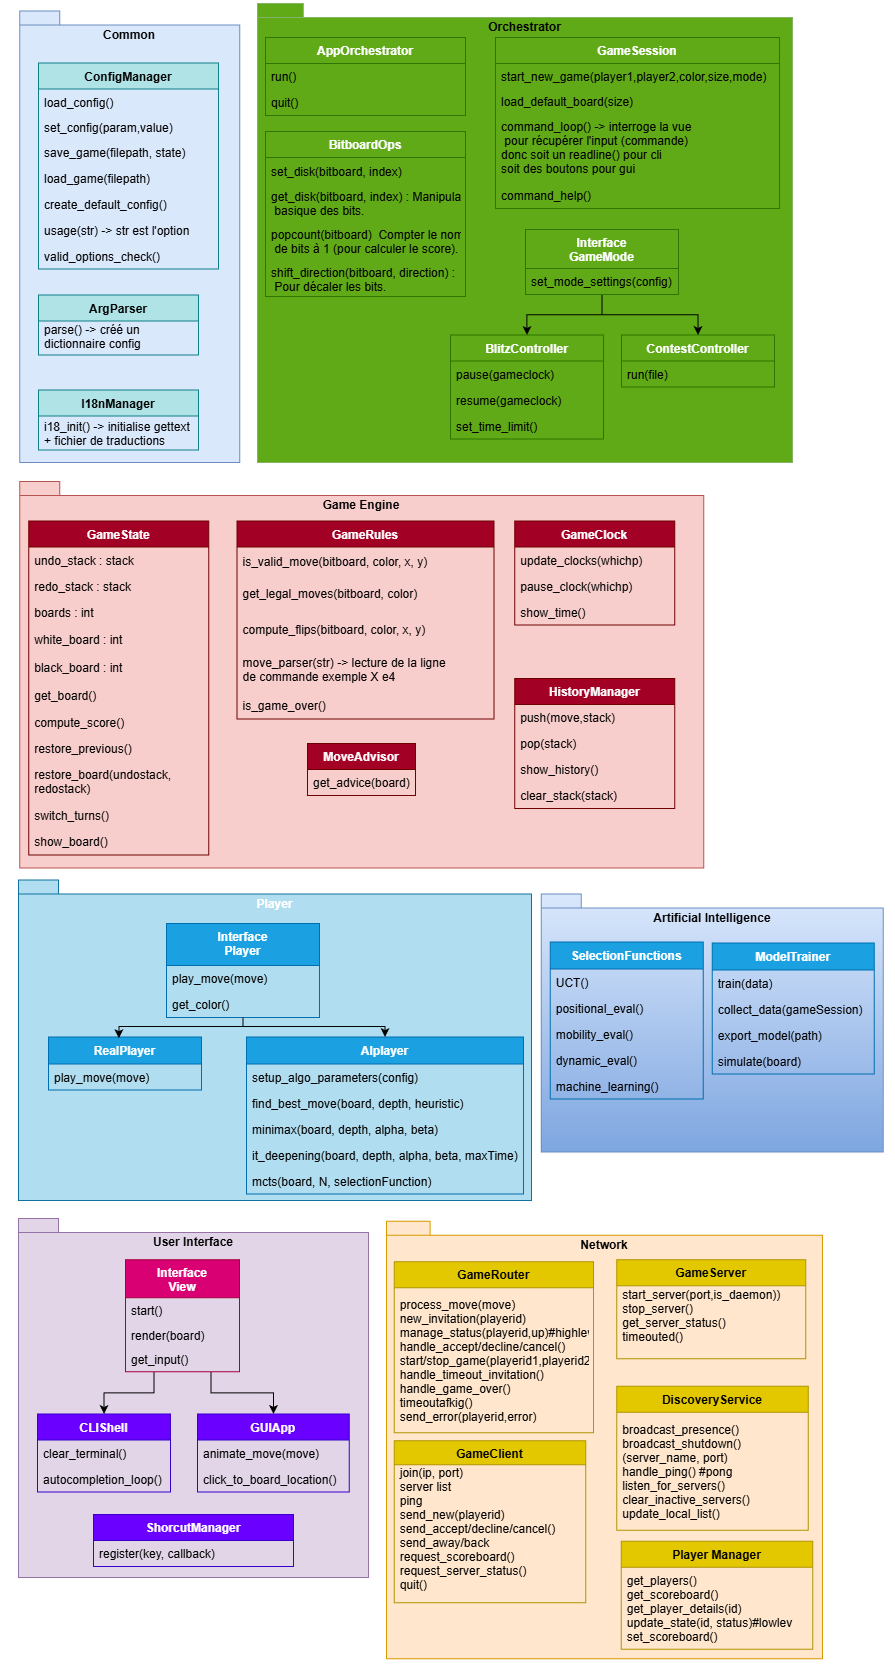
\includegraphics[scale=0.5]{architecture.png}
\caption{Classes et API}
\end{figure}
\subsection{Réseaux}
\subsubsection{Initialisation du Serveur}
Le démarrage du serveur suit une procédure stricte d'initialisation des ressources et de découverte réseau.

\begin{enumerate}
    \item \textbf{Démarrage (Bootstrap) :} L'administrateur exécute la commande \texttt{server start <port>}. Cela déclenche l'ouverture d'un \textbf{socket TCP} en mode écoute (listening) pour gérer les futures connexions entrantes.
    \item \textbf{Instanciation des Gestionnaires :} Le serveur initialise le \texttt{PlayerManager} (gestion des états des joueurs connectés) et le \texttt{Router} (aiguillage des paquets).
    \item \textbf{Notification et Découverte :} Une fois prêt, le serveur notifie l'administrateur de son succès. En parallèle, il active un mécanisme de \textbf{Broadcast} (diffusion) sur le réseau local. C'est à cet instant précis que le serveur devient visible pour les clients potentiels.
\end{enumerate}

\begin{figure}[H]
\centering
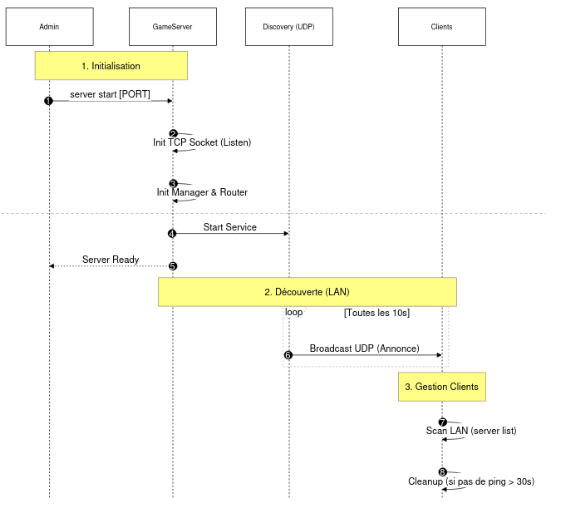
\includegraphics[scale=0.5]{Slide1_1.png}
\caption{Diagramme de séquence : Initialisation du Serveur}
\end{figure}

\subsubsection{Protocole d'Invitation et Lancement de Partie}
Le système permet à un joueur (ex: Alice) de défier un autre joueur connecté (ex: Bob). Ce processus garantit la synchronisation des états avant le début du jeu.

\begin{itemize}
    \item \textbf{Vérification d'état :} Lorsqu'Alice envoie une invitation, le serveur interroge le module \texttt{PlayerManager}. Il vérifie que la cible (Bob) est dans l'état \texttt{IDLE} (disponible).
    \item \textbf{Négociation :} Si Bob est disponible, la requête lui est transmise. S'il l'accepte, le serveur reçoit la confirmation.
    \item \textbf{Instanciation de la Session :} Le serveur initialise alors les contrôleurs spécifiques à la partie : \texttt{GameRouter} et \texttt{GameClient}.
    \item \textbf{Début de Match :} Enfin, le serveur envoie un paquet de confirmation aux deux clients, les désignant officiellement comme opposants et lançant la boucle de jeu.
\end{itemize}

\begin{figure}[H]
\centering
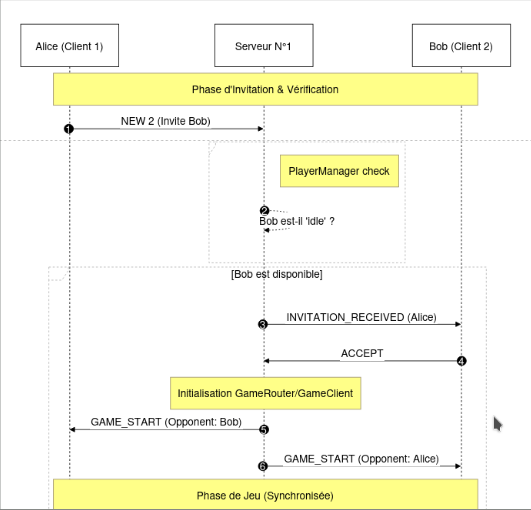
\includegraphics[scale=0.5]{Slide1_2.png}
\caption{Diagramme de séquence : Processus d'invitation}
\end{figure}

\subsubsection{Cycle de Jeu et Validation (Game Loop)}
Une fois la partie lancée, le serveur assure le rôle d'arbitre centralisé pour garantir l'intégrité de la partie. Le diagramme suivant illustre le flux de traitement d'un coup :

\begin{enumerate}
    \item \textbf{Soumission :} Le joueur actif transmet son coup au serveur.
    \item \textbf{Validation :} Le module \texttt{GameRouter} intercepte la requête et sollicite une instance de \texttt{GameRule}. Il vérifie la légalité du coup.
    \item \textbf{Transmission :} Si le coup est valide, le serveur met à jour l'état du jeu et relaie l'information à l'adversaire pour maintenir la synchronisation.
    \item \textbf{Fin de partie :} Cette boucle se répète jusqu'à la condition de victoire, moment où le serveur notifie le vainqueur aux deux participants.
\end{enumerate}

\begin{figure}[H]
\centering
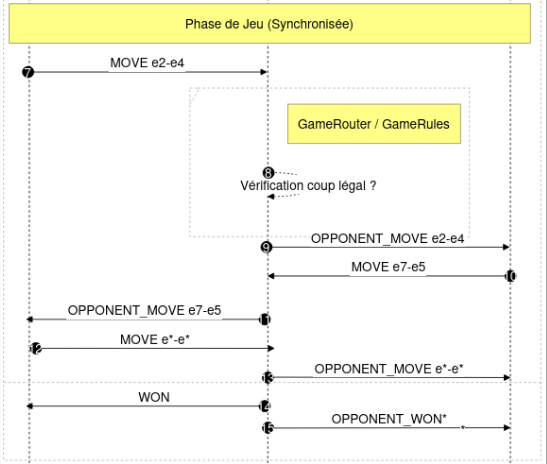
\includegraphics[scale=0.5]{Slide2_1.png}
\caption{Diagramme de séquence : Déroulement d'un coup}
\end{figure}

\subsubsection{Modèle de Concurrence (Multithreading)}
Pour supporter plusieurs parties simultanées sans blocage, le serveur implémente une architecture multithreadée (1 thread pour 2 clients).

\begin{itemize}
    \item \textbf{Isolation des sessions :} Dès que deux joueurs (A et B) s'accordent pour jouer, le serveur instancie un nouveau \textbf{Thread de Partie} dédié. Une \texttt{GameID} unique est générée et transmise aux clients.
    \item \textbf{Sécurisation des échanges :} Chaque requête client doit inclure le couple (\texttt{UserID}, \texttt{GameID}). Le thread vérifie systématiquement que le joueur appartient bien à l'instance de jeu ciblée avant de traiter l'action.
    \item \textbf{Cycle de vie :} Le thread reste actif durant toute la durée du match. À la fin de la partie, le thread est détruit pour libérer les ressources et les joueurs sont redirigés vers l'état \texttt{IDLE} (lobby principal).
\end{itemize}

\begin{figure}[H]
\centering
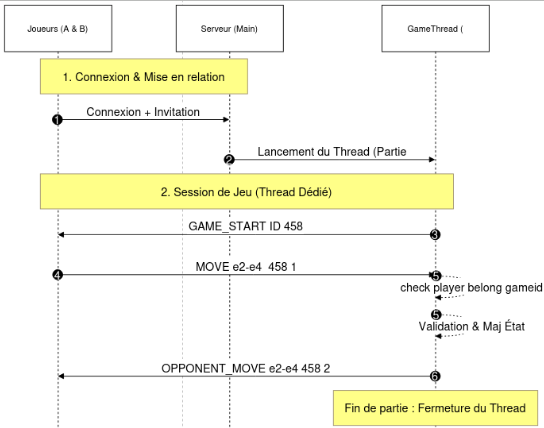
\includegraphics[scale=0.5]{Slide2_2.png}
\caption{Architecture Multithread (1 Thread / Partie)}
\end{figure}

\section{Spécifications étendues : Conseils aux joueurs (F13)}

\textbf{Besoin Visé :} F13. Gestion des conseils (Hint). Le programme doit suggérer un coup pertinent au joueur humain sur demande.

\subsection{Sous-besoins et Actions}
\begin{enumerate}
    \item \textbf{Calcul du meilleur coup :} Nécessite d'interroger le moteur d'IA sans modifier l'état actuel.
    \item \textbf{Affichage :} Le conseil doit être affiché clairement (ex: coordonnée en CLI).
\end{enumerate}

\subsection{Intégration Architecturale}
Création d'une classe \texttt{MoveAdvisor} dans le package \texttt{GameEngine} avec la méthode \texttt{get\_advice()}.
\begin{signature}{get\_advice}
    \textbf{Contexte :} Méthode de la classe \texttt{MoveAdvisor} (Package \texttt{Model}).
    
    \textbf{Prototype :}
    \begin{lstlisting}[language=Python, frame=none, numbers=none, xleftmargin=0pt, basicstyle=\ttfamily\bfseries]
def get_advice(board, game_state: GameState) -> tuple[int, int]:
    \end{lstlisting}
    
    \textbf{Entrées :}
    \begin{itemize}
        \item \texttt{game\_state} : L'état complet du jeu (plateaux et tour actuel).
    \end{itemize}
    
    \textbf{Sortie :} 
    \begin{itemize}
        \item \texttt{(x, y)} : Tuple d'entiers représentant le meilleur coup suggéré.
        \item Retourne \texttt{(-1, -1)} si aucun mouvement n'est possible.
    \end{itemize}
    
    \textbf{Description :} 
    Cette fonction analyse le plateau actuel avec une profondeur de recherche limitée pour fournir une aide rapide au joueur (commande \texttt{hint}), sans modifier l'état réel de la partie.
\end{signature}

\subsection{Scénario de Validation}

    Lancer une partie en mode CLI. Puis jouer quelques coups pour arriver à une situation connue (ex : possibilité de prendre un coin). Taper la commande \texttt{hint}. Vérifier que le programme propose le coup du coin (coup stratégique fort). Vérifier que l'état du jeu n'a pas changé (pas de coup joué automatiquement).

\section{Planning Prévisionnel}

Le projet se déroule sur 13 semaines. Voici les grandes phases :
\begin{itemize}
    \item \textbf{Phase 1 : Conception (S0-S3)} Analyse, Architecture.
    \item \textbf{Phase 2 : Développement Core (S4-S5)} Bitboards, Règles, CLI Basique.
    \item \textbf{Phase 3 : Développement Squads (S6-S8)} IA (Rémi et Matthieu), GUI (Gabriel), Réseau (Arthur et Grégory).
    \item \textbf{Phase 4 : Finalisation (S9-S12)} Revue et correction du code.
\end{itemize}


\begin{figure}[H]
    \centering
    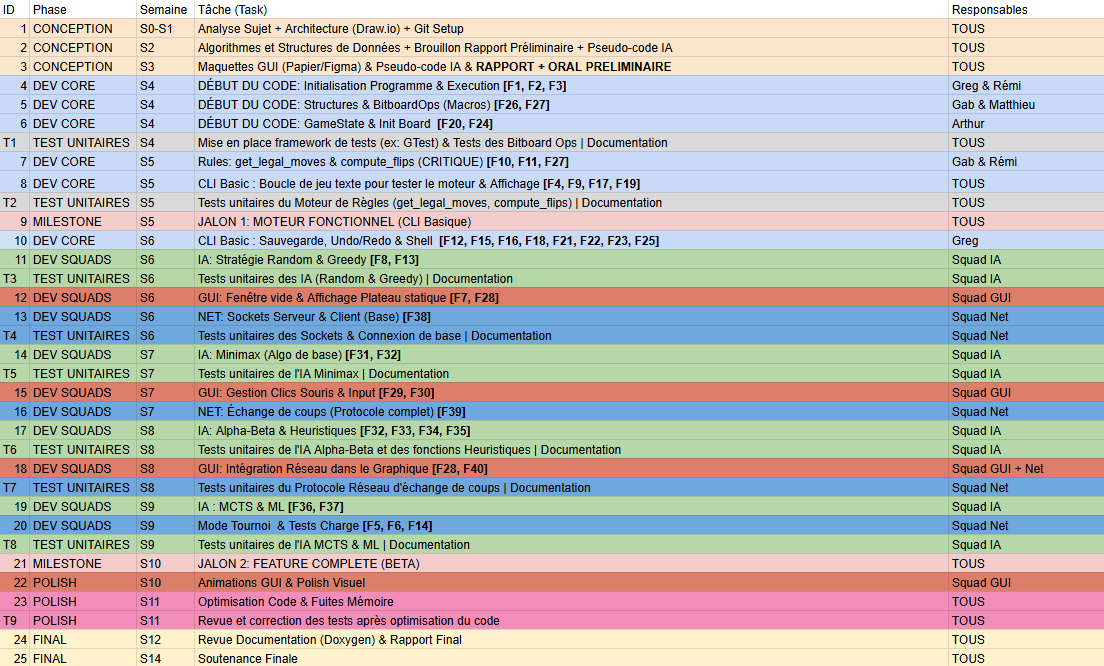
\includegraphics[width=1\linewidth]{image.png}
    \caption{Agenda du Projet}
    \label{fig:placeholder}
\end{figure}

\bibliographystyle{unsrt}
\bibliography{bibliography} 
\end{document}